% Part: sets-functions-relations
% Chapter: arithmetization
% Section:reals

\documentclass[../../../include/open-logic-section]{subfiles}

\begin{document}

\olfileid{sfr}{arith}{real}
\olsection{వాస్తవ సంఖ్యా రేఖ}

తదుపరి మెట్టు, కరణీయ సంఖ్యల నుంచి వాస్తవ సంఖ్యలను ఎలా నిర్మించాలో
చూపడం. అంతకంటే ముందు వాస్తవ సంఖ్యల \emph{విశిష్టత} ఏమిటో
అర్థం చేసుకోవాలి.

వాస్తవ సంఖ్యలు కరణీయ సంఖ్యల మాదిరిగానే చాలావరకు ప్రవర్తిస్తాయి.
(సాంకేతికంగా, రెండూ \emph{క్రమిత క్షేత్రాలకు} ఉదాహరణలు; దాని
నిర్వచనం కోసం \olref[check]{orderedfield} చూడండి.)
\olref[sfr][siz][]{chap}కు ఇచ్చిన సాధనలను మీరు పరిష్కరించి ఉంటే,
కరణీయ సంఖ్యల కంటే వాస్తవ సంఖ్యలు ఖచ్చితంగా ఎక్కువని, అంటే
$\cardless{\Rat}{\Real}$ అని మీకు తెలుసు. దీనిని మొదట కాంటర్
నిరూపించాడు. కానీ అకరణీయ సంఖ్యలు---అంటే కరణీయాలు కాని వాస్తవ
సంఖ్యలు---ఉన్నాయని సుమారు రెండున్నర సహస్రాబ్దాలుగా తెలుసు. నిజానికి:
%\footnote{ఇక్కడ ``$\sqrt{2}$'' ధన, ఋణ మూలాలు రెండింటినీ సమానంగా సూచిస్తుంది; కానీ తరువాతి కొన్ని పుటల్లో దీనిని విస్మరించి ధన మూలాన్ని మాత్రమే పరిశీలిస్తాను.}
\begin{thm}\ollabel{root2irrational}
$\sqrt{2}$ కరణీయ సంఖ్య కాదు; అంటే, $\sqrt{2} \notin \Rat$.
\end{thm}

\begin{proof}
వైరుధ్య పద్ధతిలో, $\sqrt{2}$ కరణీయమని అనుకుందాం. అప్పుడు ఏవో సహజ
సంఖ్యలు $m$, $n$లకు $\sqrt{2} = \nicefrac{m}{n}$. అంతేకాక, ఆ భిన్నాన్ని
ఇంకా కుదించలేని విధంగా $m$, $n$లను ఎంచుకోవచ్చు. పునర్వ్యవస్థీకరిస్తే
$m^{2} = 2n^{2}$. ఇక్కడి నుంచి నిరూపణను రెండు విధాలుగా పూర్తి చేయవచ్చు.

\emph{మొదట, రేఖాగణిత పద్ధతిలో} (టెనెన్‌బామ్‌ను అనుసరించి).\footnote{ఈ
నిరూపణను \cite{Conway2006} నివేదించారు.} ఈ చతురస్రాలను పరిశీలించండి:
\begin{center}
	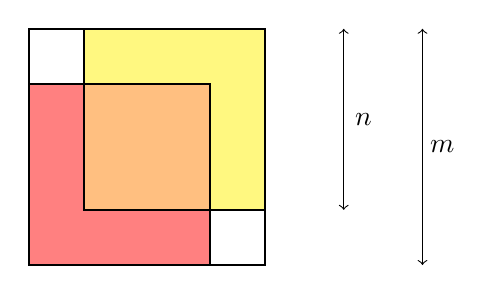
\begin{tikzpicture}
		\draw[thick] (0,0) rectangle (3,3);
		\draw[thick, fill=red!50] (0,0) rectangle (2.3,2.3);
		\draw[thick, fill=yellow!50] (0.7,0.7) rectangle (3, 3);
		\draw[thick, fill=orange!50] (0.7,0.7) rectangle (2.3, 2.3);
		\draw[<->] (4, 0.7)--(4, 3);
		\node at (4.25, 1.85) (n) {$n$};
		\draw[<->] (5, 0)--(5, 3);
		\node at (5.25, 1.5) (m) {$m$};
	\end{tikzpicture}
\end{center}
$m^2 = 2n^2$ కనుక, $n$ భుజం గల రెండు చతురస్రాలు అతివ్యాప్తి చెందే
ప్రాంత వైశాల్యం, ఆ రెండు చతురస్రాలలో ఏదీ కప్పని ప్రాంత వైశాల్యానికి
సమానం; అంటే నారింజ చతురస్ర వైశాల్యం, రంగు వేయని రెండు చతురస్రాల
వైశాల్యాల మొత్తానికి సమానం. కాబట్టి నారింజ చతురస్ర భుజం $p$, రంగు
వేయని ఒక్కొక్క చతురస్ర భుజం $q$ అయితే, $p^2 = 2q^2$. ఇప్పుడు
$\sqrt{2} = \nicefrac{p}{q}$; ఇక్కడ $p < m$, $q < n$, మరియు
$p, q \in \Nat$. ఇది $m$, $n$లను సాధ్యమైనంత చిన్నవిగా ఎంచుకున్నామనే
వాస్తవానికి విరుద్ధం.

\emph{రెండవది, లాంఛన పద్ధతిలో.} $m^{2} = 2n^{2}$ కనుక $m$ సరి సంఖ్య.
($x$ బేసి అయితే $x^2$ కూడా బేసి అని సులభంగా చూపవచ్చు.) అందువల్ల
ఏదో $r \in \Nat$కు $m = 2r$. పునర్వ్యవస్థీకరిస్తే $2r^2 = n^2$,
		%				\begin{align*}
		%					(2q)^{2} &= 2n^{2}\\
		%					4q^{2} &= 2n^{2}\\
		%					2q^{2} &= n^{2}
		%				\end{align*}
కాబట్టి $n$ కూడా సరి సంఖ్య. అందువల్ల $m$, $n$ రెండూ సరి సంఖ్యలు;
కనుక $\nicefrac{m}{n}$ భిన్నాన్ని \emph{ఇంకా} కుదించవచ్చు. వైరుధ్యం!
\end{proof}

మధ్యలో ఒక విషయం: ఈ చిత్ర ఆధారిత నిరూపణ
\olref[his][set][mythology]{sec}లోని విషయాన్ని మళ్లీ పరిశీలించడానికి
అవకాశమిస్తుంది. టెనెన్‌బామ్ (1927--2006) పూర్తిగా ఆధునిక గణితవేత్త;
అయినా ఈ నిరూపణ నిస్సందేహంగా అందమైనది, పూర్తిగా కచ్చితమైనది, రేఖాగణిత
అంతర్బుద్ధిని ఆశ్రయిస్తుంది!

ఏదేమైనా, వాస్తవ సంఖ్యలు కరణీయ సంఖ్యల కంటే ``మరింత విస్తృతమైనవి''.
ఒక అర్థంలో కరణీయ సంఖ్యల్లో ``ఖాళీలు'' ఉన్నాయి; వాటిని వాస్తవ సంఖ్యలు
పూరిస్తాయి. వాస్తవ సంఖ్యలను కరణీయ సంఖ్యల నుంచి వేరు చేసే ఒకే ధర్మాన్ని
ఇది వివరిస్తుందని వైయర్‌స్ట్రాస్ గ్రహించాడు; అదే సంపూర్ణతా ధర్మం:
\emph{ఊర్ధ్వ అవధి గల ప్రతి శూన్యేతర వాస్తవ సంఖ్యల సమితికి కనిష్ఠ
ఊర్ధ్వ అవధి ఉంటుంది.}

కరణీయ సంఖ్యలకు సంపూర్ణతా ధర్మం లేదని సులభంగా చూడవచ్చు. ఉదాహరణకు,
$\sqrt{2}$ కంటే తక్కువ కరణీయ సంఖ్యల సమితిని, అంటే దీనిని పరిశీలించండి:
\[
	\Setabs{p \in \Rat}{p^2 < 2 \text{ or }p < 0}
\]
దీనికి కరణీయ సంఖ్యల్లో ఒక ఊర్ధ్వ అవధి ఉంది; ఉదాహరణకు, దీని
!!{element}s అన్నీ $3$ కంటే చిన్నవి. కానీ దీని కనిష్ఠ ఊర్ధ్వ అవధి
ఏది? `$\sqrt{2}$' అని చెప్పాలని కోరుకుంటాం; కానీ $\sqrt{2}$
\emph{కరణీయం కాదని} ఇప్పుడే చూశాం. అంతేకాక $\sqrt{2}$ కంటే పెద్దదైన
\emph{అతి చిన్న} కరణీయ సంఖ్య లేదు. కాబట్టి ఈ సమితికి ఊర్ధ్వ అవధి
ఉంది, కానీ కనిష్ఠ ఊర్ధ్వ అవధి లేదు. అందువల్ల కరణీయ సంఖ్యలకు
సంపూర్ణతా ధర్మం లేదు.
\sourcecorrection{OLTEARITH-002}{ఆంగ్ల మూలంలో మూలకాల టోకెన్
వెంట అర్థంలేని అదనపు ``$<$'' అక్షరం ఉంది. ఇక్కడ ఆ ఒక్క ముద్రణ
దోషాన్ని తొలగించాం; ``అన్నీ $3$ కంటే చిన్నవి'' అనే వాక్యార్థం మారలేదు.}

దీనికి విరుద్ధంగా, అవిచ్ఛిన్న సమితికి సంపూర్ణతా ధర్మం ఉండటం
``సహజంగా ఉండాలి''. $\sqrt{2}$ ఒక వాస్తవ సంఖ్య కావడమే కాదు; కరణీయ
సంఖ్యా రేఖలోని ``ఖాళీలు'' అన్నింటినీ పూరించాలని కోరుకుంటాం. నిజానికి
అవిచ్ఛిన్న సమితిలోనే ``ఖాళీలు'' ఏవీ ఉండకూడదు. సంపూర్ణత ద్వారా మనకు
లభించేది సరిగ్గా ఇదే.

\end{document}
